\documentclass[border=10pt]{standalone}
\usepackage{tikz}
\usepackage{amsmath}
\usetikzlibrary{arrows.meta}

\begin{document}
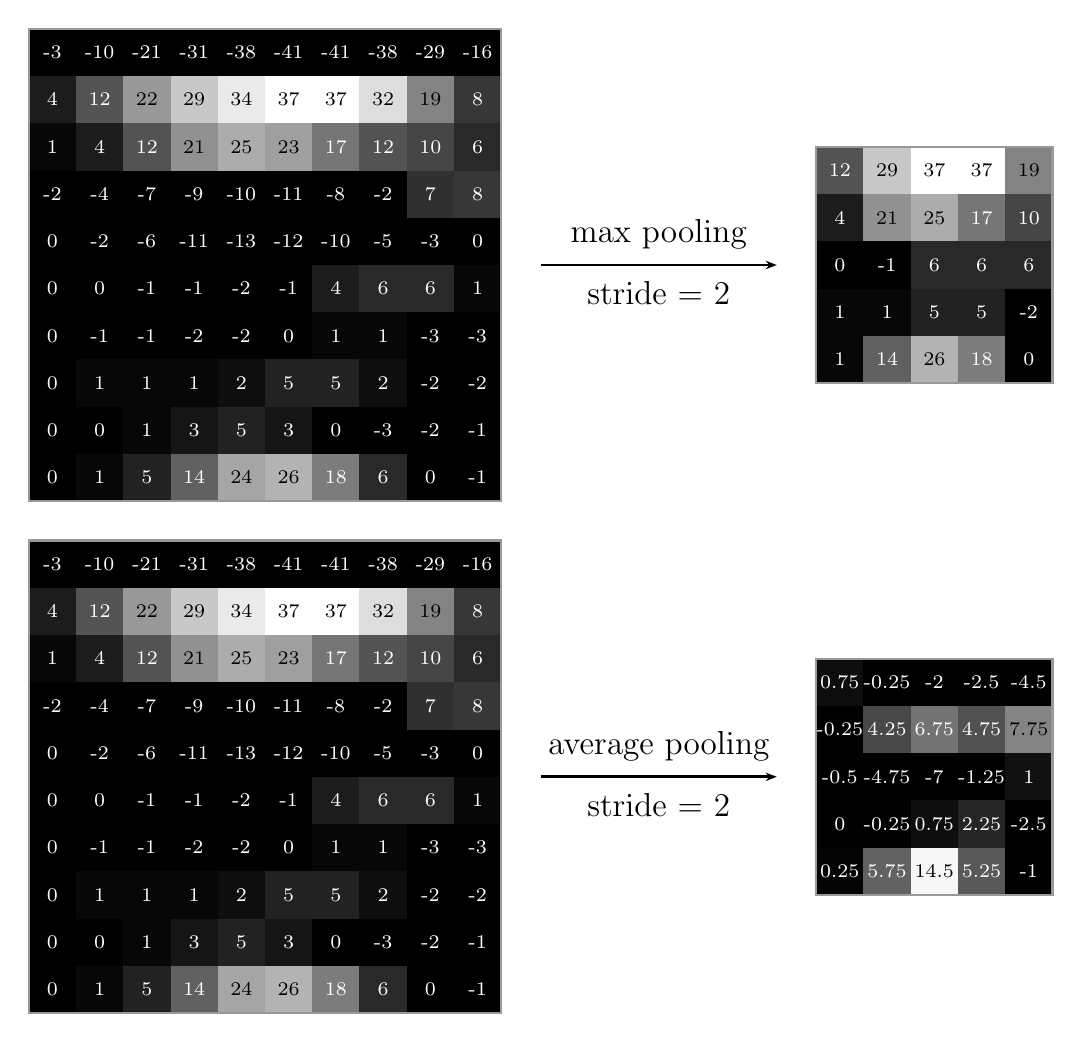
\begin{tikzpicture}[>={Stealth[length=4pt]}, line width=0.8pt, font=\large]

  % ========== 可复用：NxN 灰度图（全填充；#2=N, #3=x, #4=y, #5=值；可选#1=灰度满量程，默认37） ==========
  \newcommand{\drawresultfull}[5][37]{%
    \foreach \v [count=\n] in {#5} {%
      \pgfmathtruncatemacro{\r}{int((\n-1)/#2)}
      \pgfmathtruncatemacro{\c}{int(mod(\n-1,#2))}
      \pgfmathsetmacro{\g}{max(0, min(\v/#1, 1))}
      \definecolor{oc}{gray}{\g}
      \ifdim\g pt>0.5pt \def\tc{black}\else \def\tc{white}\fi
      \fill[oc] ({#3+0.6*\c}, {#4+0.6*(#2-1-\r)}) rectangle ++(0.6,0.6);
      \node[font=\scriptsize, text=\tc] at ({#3+0.6*\c+0.3}, {#4+0.6*(#2-1-\r)+0.3}) {\v};
    }%
    \draw[gray!80] (#3,#4) rectangle ({#3+0.6*#2}, {#4+0.6*#2});
  }

  % ================= 第一行：max pooling =================
  \drawresultfull{10}{0}{7}{%
    -3,-10,-21,-31,-38,-41,-41,-38,-29,-16,%
    4,12,22,29,34,37,37,32,19,8,%
    1,4,12,21,25,23,17,12,10,6,%
    -2,-4,-7,-9,-10,-11,-8,-2,7,8,%
    0,-2,-6,-11,-13,-12,-10,-5,-3,0,%
    0,0,-1,-1,-2,-1,4,6,6,1,%
    0,-1,-1,-2,-2,0,1,1,-3,-3,%
    0,1,1,1,2,5,5,2,-2,-2,%
    0,0,1,3,5,3,0,-3,-2,-1,%
    0,1,5,14,24,26,18,6,0,-1}
%   \draw[red, line width=1.4pt] (4.8,7) rectangle (6,8.2);       % 右下 2x2 窗
  \draw[->, line width=1pt] (6.5,10) -- (9.5,10)
    node[midway, above=2pt] {max pooling}
    node[midway, below=2pt] {stride = 2};
  \drawresultfull{5}{10}{8.5}{%
    12,29,37,37,19,%
    4,21,25,17,10,%
    0,-1,6,6,6,%
    1,1,5,5,-2,%
    1,14,26,18,0}
%   \draw[red, line width=1.4pt] (12.4,8.5) rectangle (13,9.1);   % 对应右下格 = 0

  % ================= 第二行：average pooling（同一输入、同一红窗） =================
  \drawresultfull{10}{0}{0.5}{%
    -3,-10,-21,-31,-38,-41,-41,-38,-29,-16,%
    4,12,22,29,34,37,37,32,19,8,%
    1,4,12,21,25,23,17,12,10,6,%
    -2,-4,-7,-9,-10,-11,-8,-2,7,8,%
    0,-2,-6,-11,-13,-12,-10,-5,-3,0,%
    0,0,-1,-1,-2,-1,4,6,6,1,%
    0,-1,-1,-2,-2,0,1,1,-3,-3,%
    0,1,1,1,2,5,5,2,-2,-2,%
    0,0,1,3,5,3,0,-3,-2,-1,%
    0,1,5,14,24,26,18,6,0,-1}
%   \draw[red, line width=1.4pt] (4.8,0.5) rectangle (6,1.7);     % 同一个 2x2 窗
  \draw[->, line width=1pt] (6.5,3.5) -- (9.5,3.5)
    node[midway, above=2pt] {average pooling}
    node[midway, below=2pt] {stride = 2};
  % 平均池化结果（灰度满量程改 15，避免整片发黑；数值为精确均值）
  \drawresultfull[15]{5}{10}{2.0}{%
    0.75,-0.25,-2,-2.5,-4.5,%
    -0.25,4.25,6.75,4.75,7.75,%
    -0.5,-4.75,-7,-1.25,1,%
    0,-0.25,0.75,2.25,-2.5,%
    0.25,5.75,14.5,5.25,-1}
%   \draw[red, line width=1.4pt] (12.4,2.0) rectangle (13,2.6);   % 对应右下格 = -1
\end{tikzpicture}
\end{document}